	\section{Получение и первичная обработка данных}
	
	
			\begin{wrapfigure}[17]{l}{0.6\linewidth}
\singlespacing
\vspace{-35px}
%  \begin{center}
    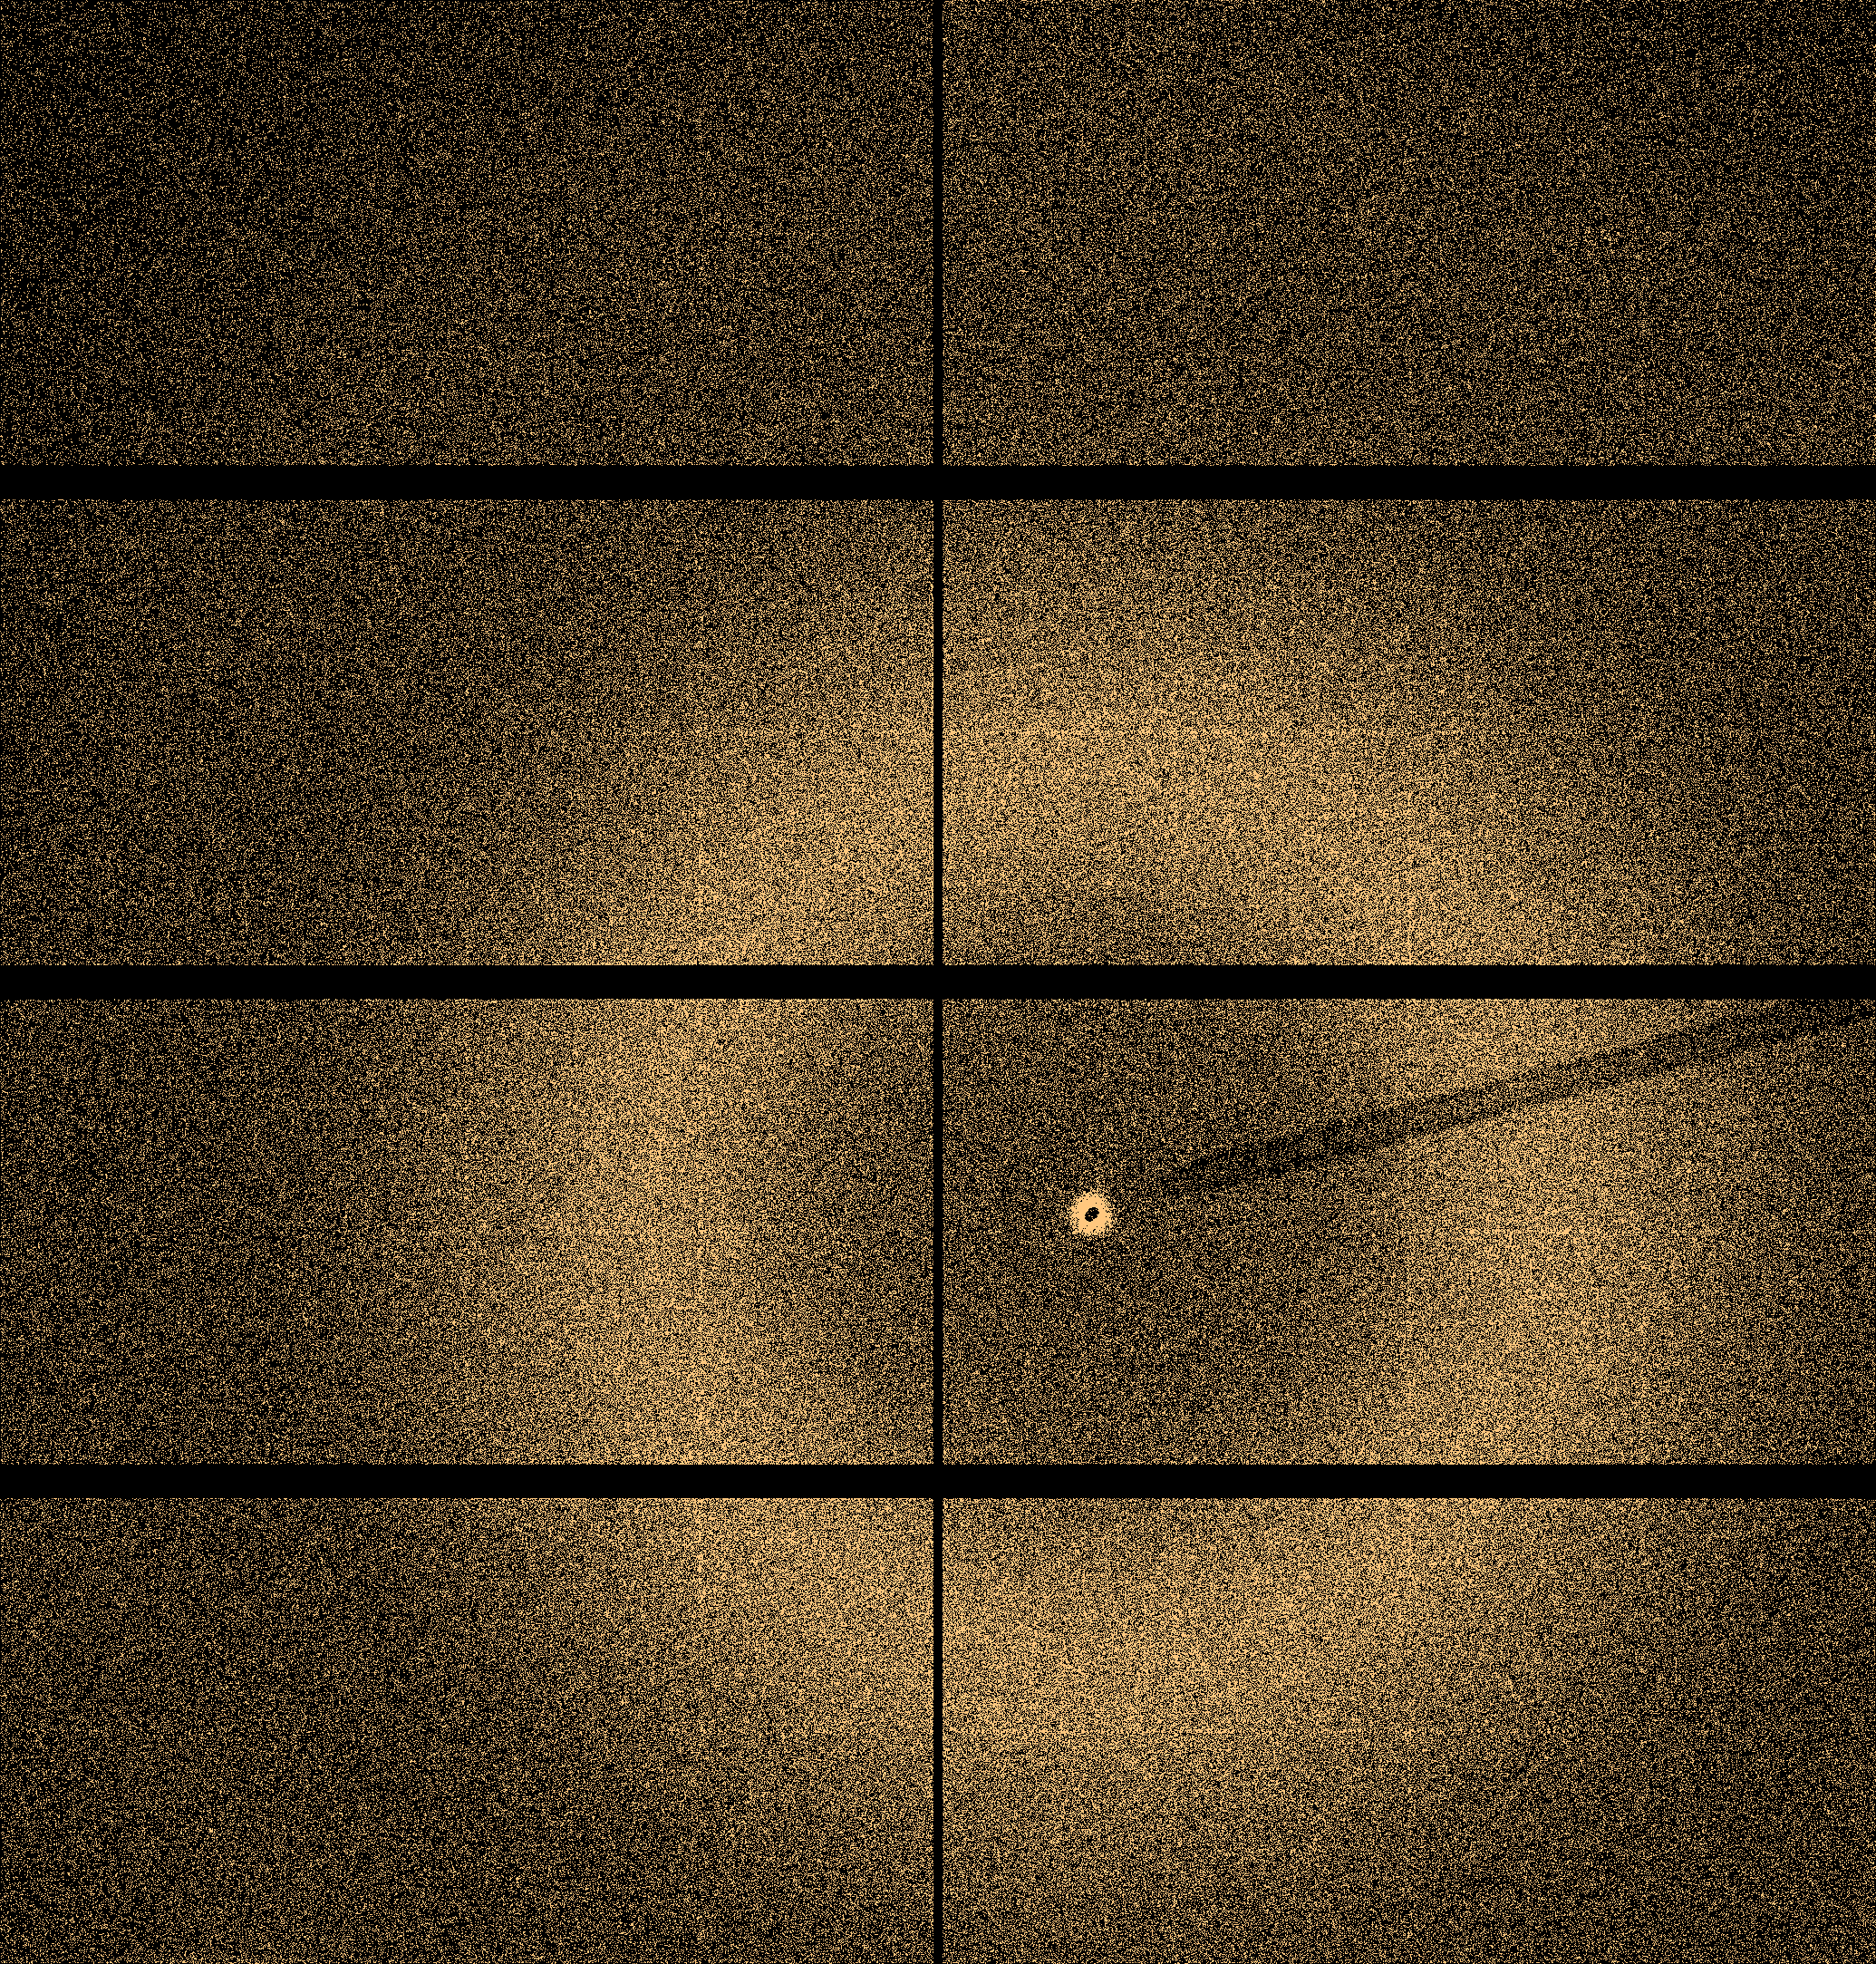
\includegraphics[width=0.9\linewidth]{fig/obj.png}
    \vspace{3px}
    \caption{Изображение с 2D~-детектора. Черные области соответствуют промежуткам между элементами детектора, затемненная облась справа  - тень от заслонки}
    \label{fig:difractogram}
%  \end{center}
\end{wrapfigure}
	
	
	Детектирование картин дифракции при сканировании образца наноразмерным пучком рентгеновского синхротронного излучения производится с шагом 1 мкм. 
	Это позволяет установить, что изучаемые порошки и пленки не являются однородными, а имеют как чисто аморфные, так и частично-кристаллические участки.
	Типичное изображение, получаемое на детекторе для единичного измерения, представлено на рис. \ref{fig:difractogram}. Различие в сигналах кристаллических и аморфных областей хорошо видно на фрагментах дифрактограмм, преобразованных к полярной системе координат, представленных на рис. \ref{fig:azim}. Как видно из рисунка, наличие кристаллической фазы приводит к появлению  дифракционных пиков, в то время как рассеяние на чисто аморфных участках дает только так называемое аморфное гало.
	
		\begin{figure}[t]\center
\begin{tabular}{cc}
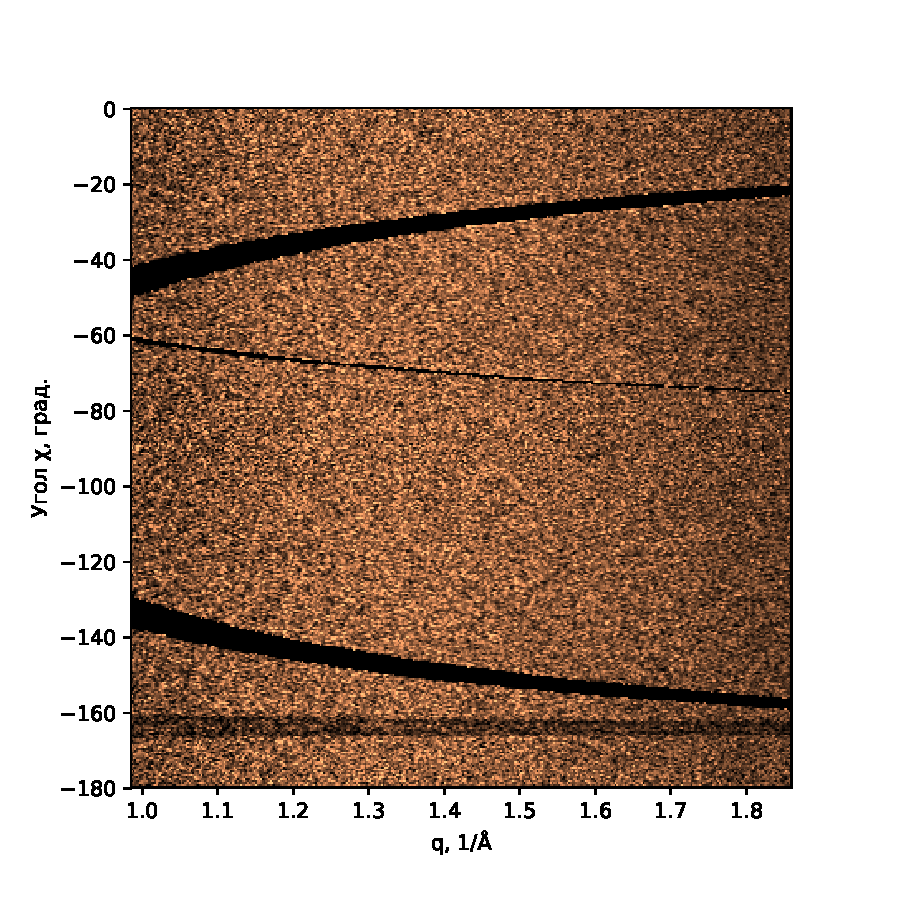
\includegraphics[width=0.5\linewidth]{fig/azim-amo.pdf}
&
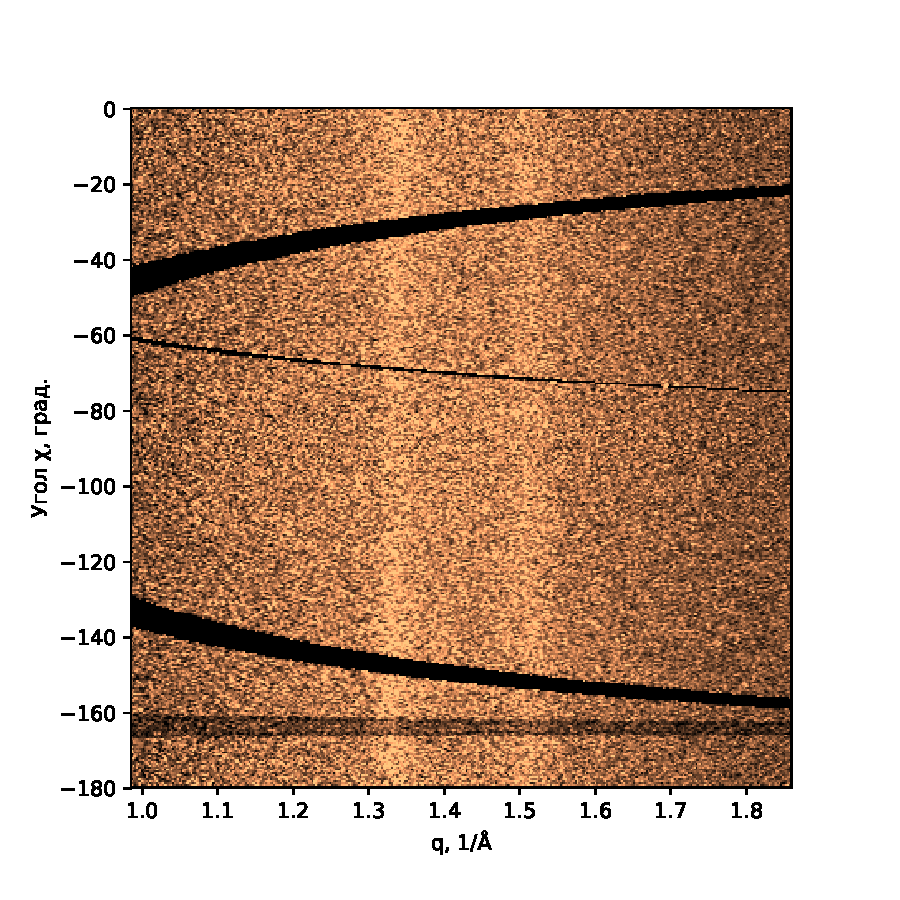
\includegraphics[width=0.5\linewidth]{fig/azim-cryst.pdf}
\end{tabular}
\caption{Фрагменты дифрактограмм (в координатах $(q,\chi)$) в аморфной (слева) и кристаллической (справа) областях.}
\label{fig:azim}
\end{figure}
	
После калибровки, в результате интегрирования по азимутальному углу $\chi$, получаются одномерные профили дифракции. Один из профилей в частично-кристаллической области в широкоугловом диапазоне представлен не рис. \ref{fig:waxs_profile}.

\begin{figure}[h]
    \centering
    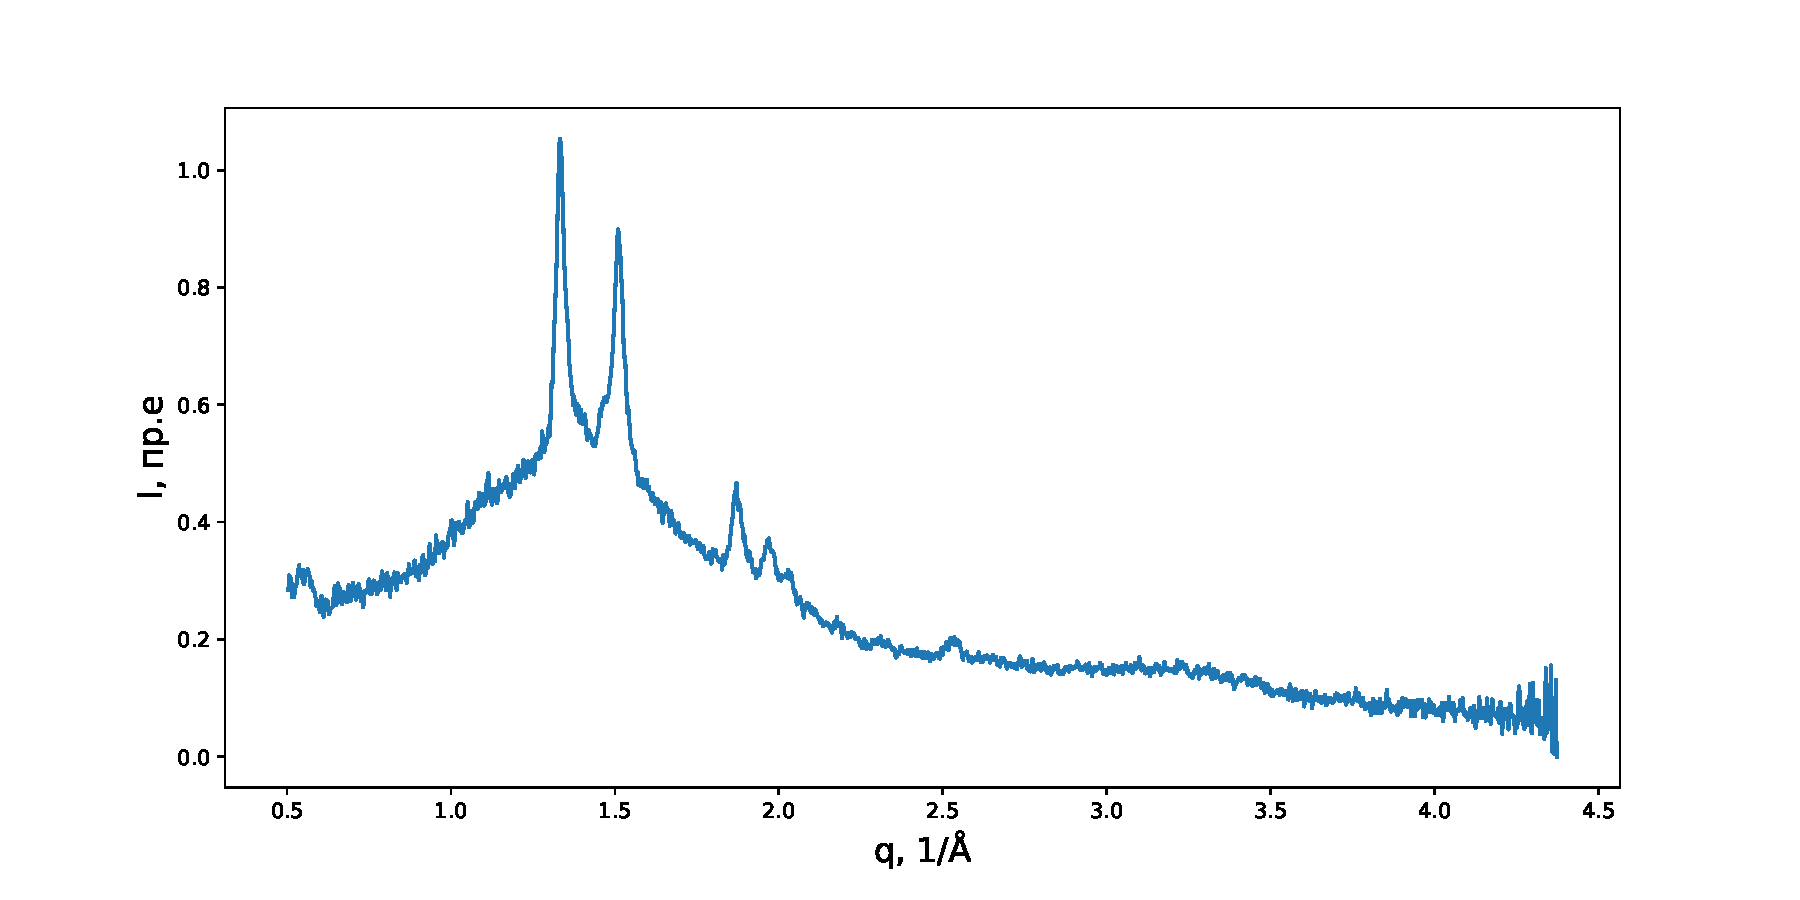
\includegraphics[width=\linewidth]{fig/profile.pdf}
    \caption{Картина дифракции в частично-кристаллической области после азимутального интегрирования}
    \label{fig:waxs_profile}
\end{figure}


	\section{Вычитание фона}
	
	Для расчета индекса кристалличности при обработке данных дифракции необходимо распознание кристаллических пиков, сигнала от аморфной фазы и фона, соответствующего рассеянию на окружающем газе и другим артефактам.
	
	В отличие от обычного фона, широкие пики рассеяния от аморфной фазы нельзя определить один раз для всех измерений, так как его форма зависит от степени кристалличности. Таким образом, его оценку необходимо проводить для каждого профиля отдельно.
	Стандартные алгоритмы для автоматического распознавания фона, основанные на полиномиальной аппроксимации, показали себя неэффективными в нашем случае. Распознавание кристаллических пиков и аморфного фона производилось с помощью фильтра "rolling ball". В рентгеноструктурном анализе он как правило применяется к двумерным дифрактограммам кристаллических материалов, как например, в работе \cite{ball2018}. Однако подходящая реализация для одномерных профилей, не представлена в открытых источниках. Ниже (листинг \ref{lst:ball}) приведена реализация алгоритма для одномерных профилей на языке Python, которая применяется далее для определения кристалличности исследуемых образцов.
	 
\vspace{5px}
	\begin{lstlisting}[language=Python, caption=Алгоритм распознавания фона, label={lst:ball}]
import numpy as np

def rolling_ball(profile, r):
    #r - ball radius
    #profile - 1D profile, smoothed
    t1 = np.full(profile.shape[0], np.amax(profile), dtype=np.float32)
    for i in range (t1.shape[0]):
        for j in range(-r,r):
            if ((i+j)>0 and (i+j)<t1.shape[0]):
                if(t1[i]>profile[i+j]):
                    t1[i]=profile[i+j]
                    
    t2 = np.zeros(profile.shape[0],dtype=np.float32)
    count = np.zeros(profile.shape[0],dtype=np.float32)
    back = np.zeros(profile.shape[0],dtype=np.float32) 
    
    for i in range(t2.shape[0]): 
        for j in range(-r,r):
            if ((i+j)>0 and (i+j)<t2.shape[0]):
                t2[i]+=t1[i+j]
                count[i]+=1
        back[i] = t2[i]/count[i]
    return back
 

\end{lstlisting}
\vspace{5px}

	Принцип действия алгоритма проиллюстрирован на рис. \ref{fig:ball}. 
	Его можно представить как круг заданного радиуса, который "катится"  под графиком \cite{ball2018}.Траектория его центра образует линию, которая и вычитается из начального профиля. 
		\begin{figure}[ht]
	    \centering
	    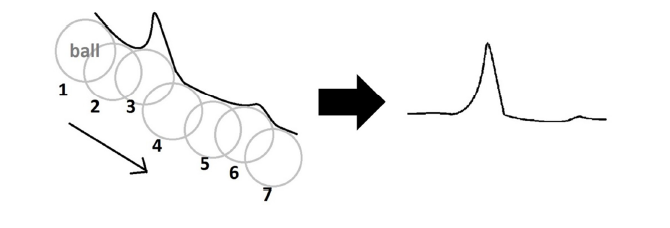
\includegraphics[width=\linewidth]{fig/ball.PNG}
	    \caption{Процедура вычитания фона.}
	    \label{fig:ball}
	\end{figure}

	
	Пики, чья ширина меньше радиуса круга, не вычитаются, и остаются в конечном профиле. Так, алгоритм позволяет убирать широкий сигнал рассеяния аморфной фазы, и оставлять только узкие кристаллические пики (рис. \ref{fig:ball-profile}).
	
	


	\begin{figure}[ht]
	    \centering
	    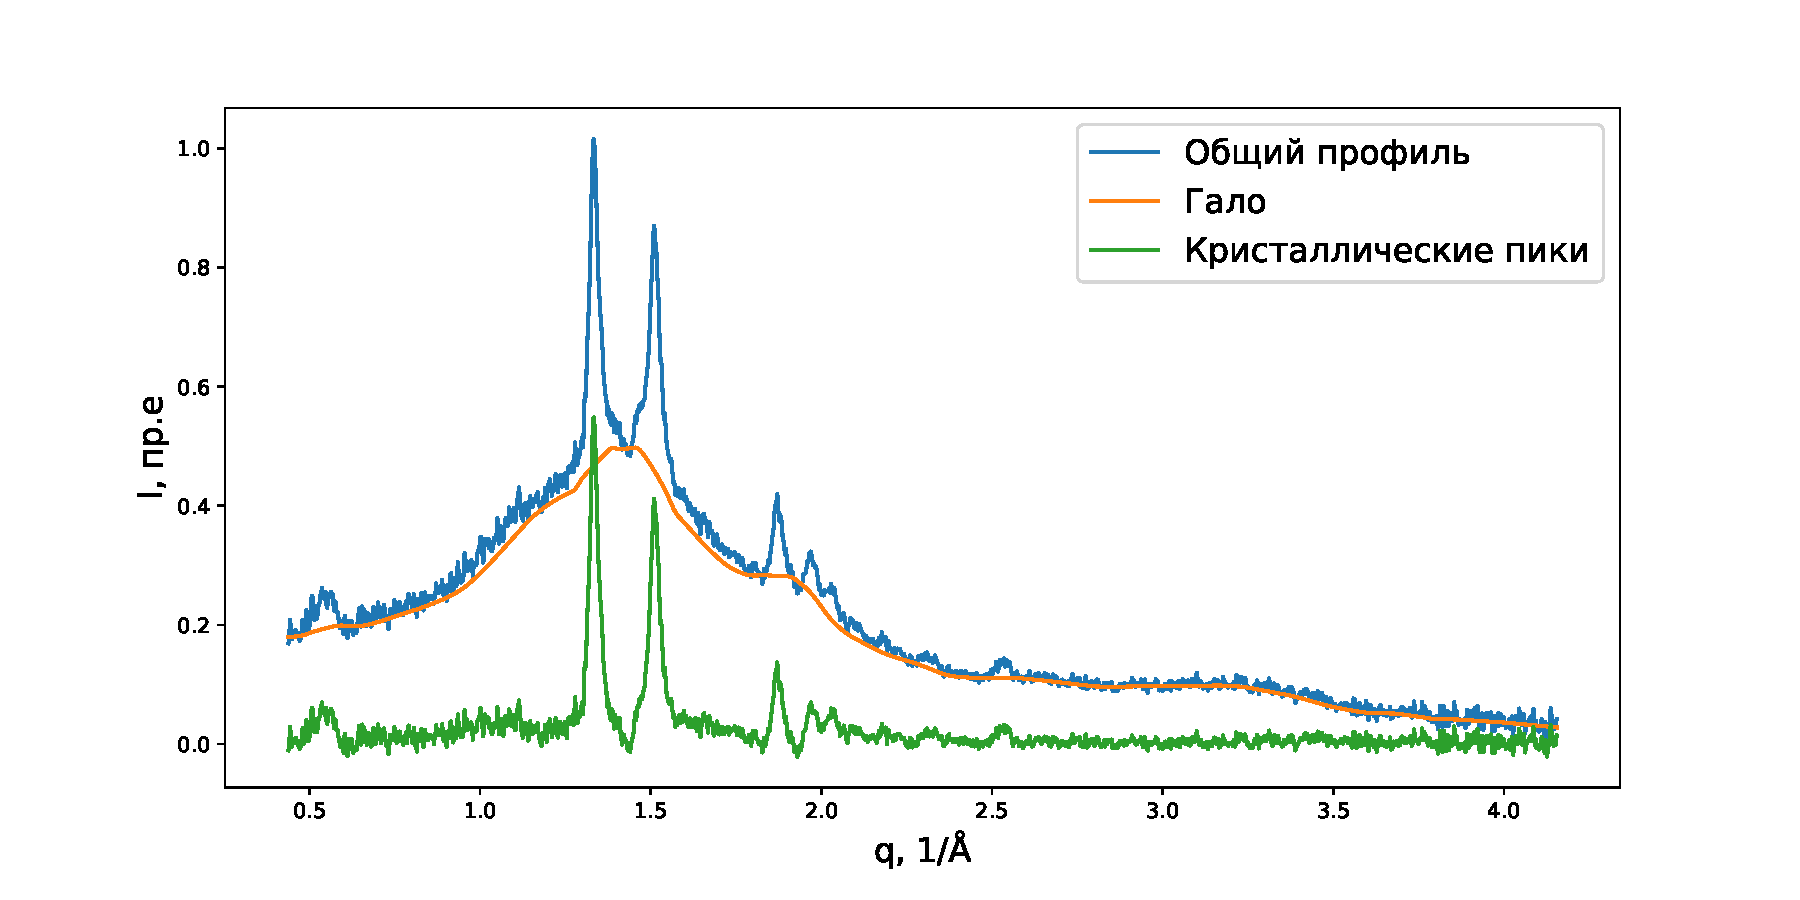
\includegraphics[width=\linewidth]{fig/ball-profile.pdf}
	    \caption{Распознавание аморфного гало}
	    \label{fig:ball-profile}
	\end{figure}



\section{Пики}

	обработка одного профиля моим алгоритмом
	
	положения пиков
	
	

\section{Картография образцов}

\subsection{Порошки}

--> Сборные карты по отдельным пикам.



\begin{figure}[h]
    \centering
    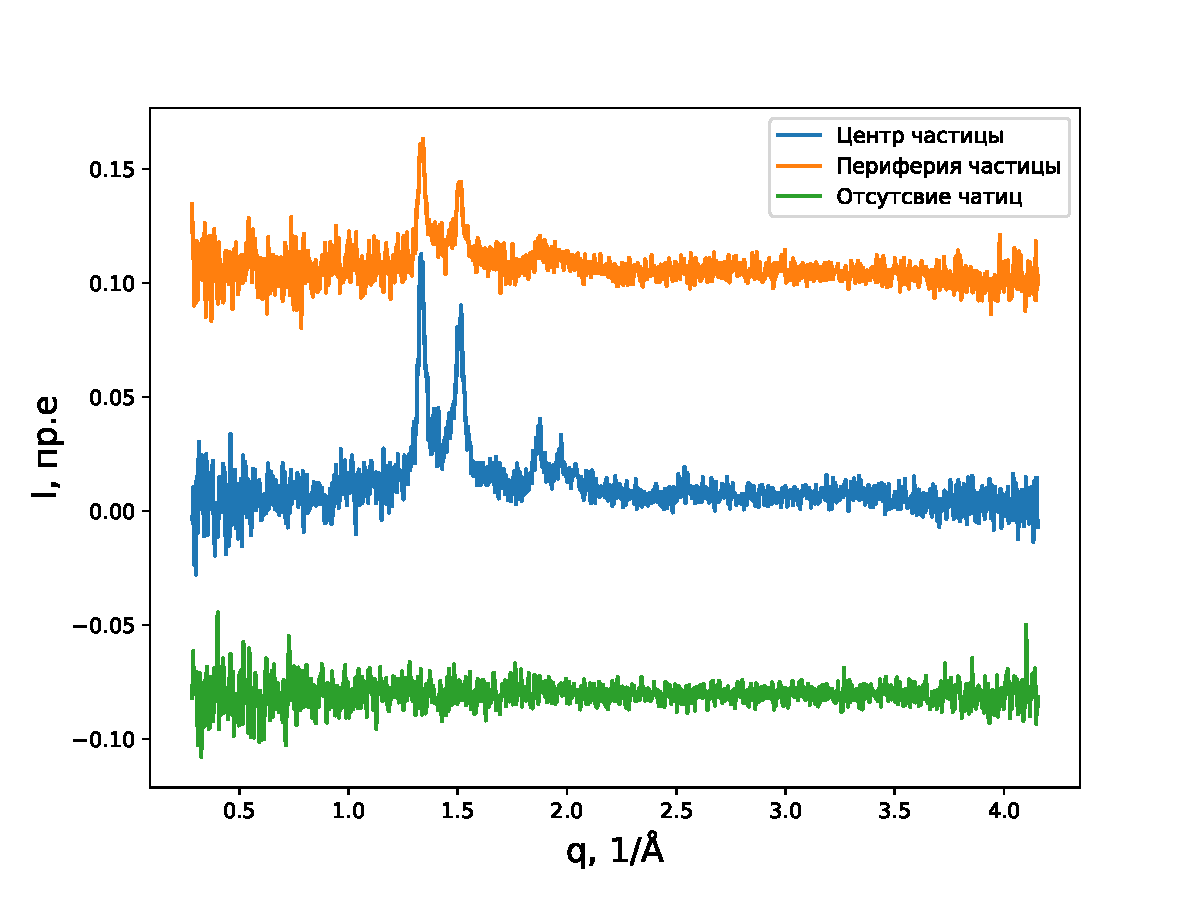
\includegraphics[width = \linewidth]{fig/var-profile.pdf}
    \caption{Профили для разных областей сканирования порошка}
    \label{fig:var-profile}
\end{figure}


	
	\paragraph{Частицы порошков.}Составление карт кристалличности образцов показывает, что сами порошки состоят из частичнокристаллических частиц заявленных размеров.
	
	\begin{figure}[h]
	    \centering
	    \begin{tabular}{ccc}
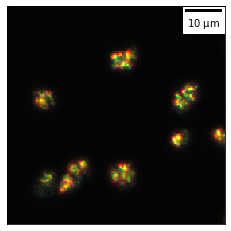
\includegraphics[width=0.33\linewidth]{fig/powder_optic.png}
&
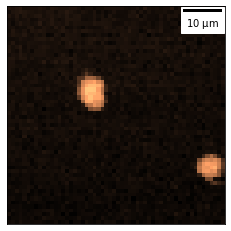
\includegraphics[width=0.33\linewidth]{fig/powder_dif1.png}
&
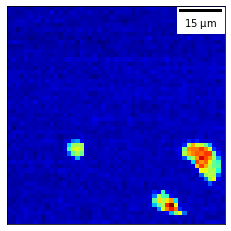
\includegraphics[width=0.33\linewidth]{fig/powder_dif2.png}
\end{tabular}
	    \caption{Отдельные частицы}
	    \label{fig:powder}
	\end{figure}
	
	\paragraph{Область SAXS.}
	\paragraph{Область WAXS.}
	
	
	
		\begin{figure}[ht]\centering
\begin{tabular}{cc}
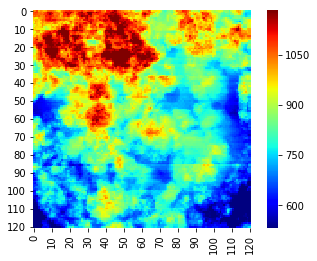
\includegraphics[width=0.5\linewidth]{fig/example72.png}
&
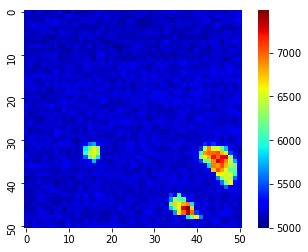
\includegraphics[width=0.5\linewidth]{fig/example1434.png} \\
\end{tabular}
\caption{Карты кристалличности}
\end{figure}
	
	
	
	
\section{Расчет характеристик}
